%
% This is the LaTeX template file for lecture notes for CS294-8,
% Computational Biology for Computer Scientists.  When preparing 
% LaTeX notes for this class, please use this template.
%
% To familiarize yourself with this template, the body contains
% some examples of its use.  Look them over.  Then you can
% run LaTeX on this file.  After you have LaTeXed this file then
% you can look over the result either by printing it out with
% dvips or using xdvi.
%
% This template is based on the template for Prof. Sinclair's CS 270.

\documentclass[twoside]{article}
\usepackage{graphics}
\usepackage{amsmath}
\usepackage{amssymb}
\usepackage{hyperref}
\usepackage{IEEEtrantools}
\usepackage{graphicx}

\setlength{\oddsidemargin}{0.25 in}
\setlength{\evensidemargin}{-0.25 in}
\setlength{\topmargin}{-0.6 in}
\setlength{\textwidth}{6.5 in}
\setlength{\textheight}{8.5 in}
\setlength{\headsep}{0.75 in}
\setlength{\parindent}{0 in}
\setlength{\parskip}{0.1 in}

%
% The following commands set up the lecnum (lecture number)
% counter and make various numbering schemes work relative
% to the lecture number.
%
\newcounter{lecnum}
\renewcommand{\thepage}{\thelecnum-\arabic{page}}
\renewcommand{\thesection}{\thelecnum.\arabic{section}}
\renewcommand{\theequation}{\thelecnum.\arabic{equation}}
\renewcommand{\thefigure}{\thelecnum.\arabic{figure}}
\renewcommand{\thetable}{\thelecnum.\arabic{table}}

%
% The following macro is used to generate the header.
%
\newcommand{\lecture}[4]{
   \pagestyle{myheadings}
   \thispagestyle{plain}
   \newpage
   \setcounter{lecnum}{#1}
   \setcounter{page}{1}
   \noindent
   \begin{center}
   \framebox{
      \vbox{\vspace{2mm}
    \hbox to 6.28in { {\bf CMPUT 652: Reinforcement Learning with Robots
                        \hfill Fall 2019} }
       \vspace{4mm}
       \hbox to 6.28in { {\Large \hfill Lecture #1: #2  \hfill} }
       \vspace{2mm}
       \hbox to 6.28in { {\it Instructor: #3 \hfill Scribe: #4} }
      \vspace{2mm}}
   }
   \end{center}
   \markboth{Lecture #1: #2}{Lecture #1: #2}
   {\bf Disclaimer}: {\it These notes have not been subjected to the
   usual scrutiny reserved for formal publications.  They may be distributed
   outside this class only with the permission of the Instructor.}
   \vspace*{4mm}
}

%
% Convention for citations is authors' initials followed by the year.
% For example, to cite a paper by Leighton and Maggs you would type
% \cite{LM89}, and to cite a paper by Strassen you would type \cite{S69}.
% (To avoid bibliography problems, for now we redefine the \cite command.)
% Also commands that create a suitable format for the reference list.
\renewcommand{\cite}[1]{[#1]}
\def\beginrefs{\begin{list}%
        {[\arabic{equation}]}{\usecounter{equation}
         \setlength{\leftmargin}{2.0truecm}\setlength{\labelsep}{0.4truecm}%
         \setlength{\labelwidth}{1.6truecm}}}
\def\endrefs{\end{list}}
\def\bibentry#1{\item[\hbox{[#1]}]}

%Use this command for a figure; it puts a figure in wherever you want it.
%usage: \fig{NUMBER}{SPACE-IN-INCHES}{CAPTION}
\newcommand{\fig}[3]{
			\vspace{#2}
			\begin{center}
			Figure \thelecnum.#1:~#3
			\end{center}
	}
% Use these for theorems, lemmas, proofs, etc.
\newtheorem{theorem}{Theorem}[lecnum]
\newtheorem{lemma}[theorem]{Lemma}
\newtheorem{proposition}[theorem]{Proposition}
\newtheorem{claim}[theorem]{Claim}
\newtheorem{corollary}[theorem]{Corollary}
\newtheorem{definition}[theorem]{Definition}
\newenvironment{proof}{{\bf Proof:}}{\hfill\rule{2mm}{2mm}}

% **** IF YOU WANT TO DEFINE ADDITIONAL MACROS FOR YOURSELF, PUT THEM HERE:

%%===========================================================================
%% defining the expectation operator
%%---------------------------------------------------------------------------
\DeclareMathOperator{\E}{\mathbb{E}}
%%===========================================================================

\begin{document}
%FILL IN THE RIGHT INFO.
%\lecture{**LECTURE-NUMBER**}{**DATE**}{**LECTURER**}{**SCRIBE**}
\lecture{7}{September 24}{Rupam Mahmood}{Yufeng Yuan}
%\footnotetext{These notes are partially based on those of Nigel Mansell.}

% **** YOUR NOTES GO HERE:

% Some general latex examples and examples making use of the
% macros follow.  
%**** IN GENERAL, BE BRIEF. LONG SCRIBE NOTES, NO MATTER HOW WELL WRITTEN,
%**** ARE NEVER READ BY ANYBODY.

\section{Last Lecture}
Previously, we understood reinforcement learning from the perspective of mind and from the first principle, we derived function approximation. The cases we encountered so far is the bandits, and a general formalization for reinforcement learning is introduced here.

\section{Finite Markov Decision Process}

Finite Markov Decision Process can be defined by a 5-tuple $\big<\mathcal{S}, \mathcal{A}, \mathcal{R}, p, \gamma \big>$ and they are states, action space, reward, transition probabilities and discount rate respectively. 


\subsection{Agent-Environment Interaction}

\begin{figure}[!hbp]
	\centering
	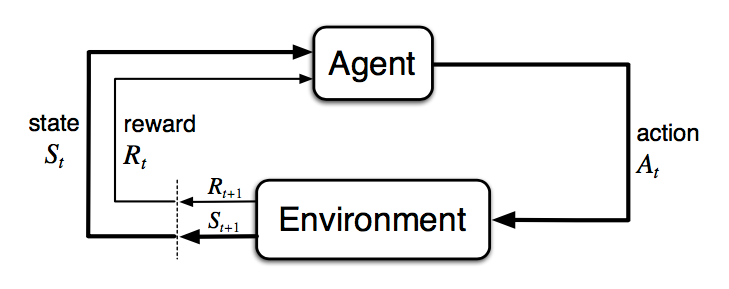
\includegraphics[scale=0.4]{images/agent_env_interaction.png}
	\caption{The agent-environment interaction in a Markov decision process}
\end{figure}

This interaction can be described as following: at each time step $t$, the agent receives some representation of the environment's state, $S_t\in\mathcal{S}$, and on that basis selects an action $A_t\in\mathcal{A}(s)$. One time step later, in part as a consequence of its action, the agent receives a numerical reward $R_{t+1}\in\mathcal{R}$, and finds itself in a new state $S_{t+1}$. Thus, the interaction of the agent and the environment will form a sequence or trajectory like: $S_0, A_0, R_1, S_1, A_1, R_2, S_2, A_2, R_3, \cdots$.

\subsection{Transition Probabilities and Return}
The transition probabilities, also known as the dynamics of MDPs, are denoted by $p$:
$$
p(s',r|s,a)=Pr\{S_t=s', R_t=r|S_{t-1}=s, A_{t-1}=a\}
$$
If $p$ is known, one should be able to compute anything else about the environment because $ p $completely characterizes the environment's dynamics. One thing should be noted here is that we assumed Markov Property here which future states is totally determined by current states.

At each time step, the goal of the agent is to maximize the cumulative future rewards which is defined as $G_t = R_{t+1} + R_{t+2} + R_{t+3} + \dots + R_T$, where $T$ is the final step. However, such formula doesn't apply to continuing tasks, where $T=\infty$, because $G_t$ will be infinity too. To unify both episodic and continuing tasks, discount is introduced:
$$
G_t = R_{t+1} + \gamma R_{t+2} + \gamma^2 R_{t+3} + \dots = \sum^\infty_{k=0}\gamma^kR_{t+k+1}
$$
where $\gamma$ is a parameter $0 \leq \gamma \leq 1$ called the discount rate. The above can also be written in recursive form: $G_t=R_{t+1}+\gamma G_{t+1}$


\subsection{A Small Example of MDP}

\begin{figure}[!hbp]
  \centering
  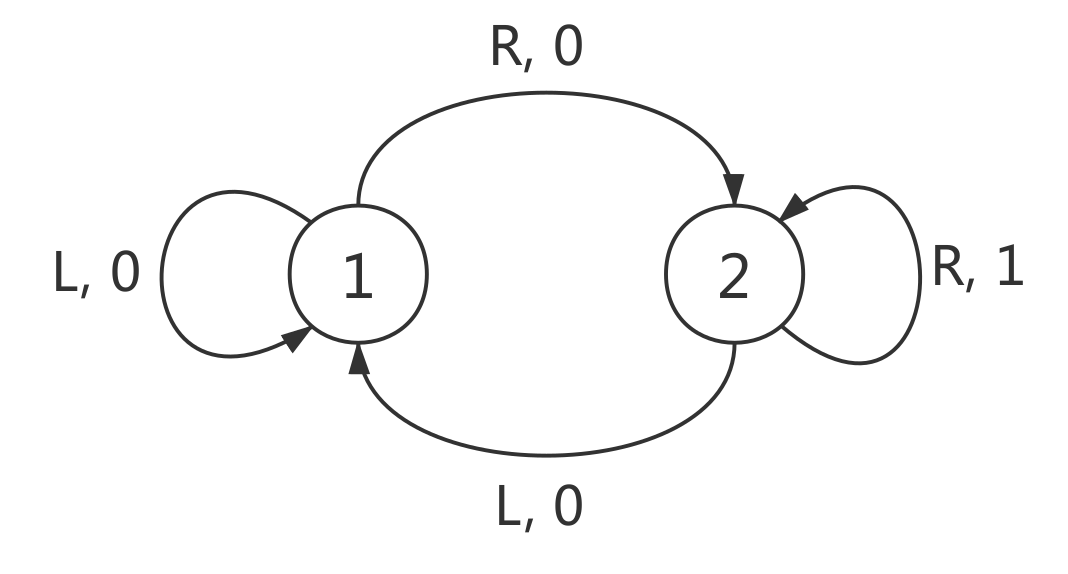
\includegraphics[scale=0.2]{images/mdp.png}
  %\caption{A learning scenario where the space of parameterized functions doesn't contain the ideal function $f^*$. In such cases, the function closest to $f^*$ is found instead.}
  \label{fig: function_space}
\end{figure}
\begin{center}
	$\gamma=0.9$
\end{center}
\begin{table}[htb!]
\centering
\begin{tabular}{c|cccc}
\hline
$p(s', r|s,a)$ & 1,0 & 1,1 & 2,0 & 2,1 \\
\hline
$p(\cdot, \cdot|1, L)$ & 1 & 0 & 0 & 0 \\
\hline
$p(\cdot, \cdot|1, R)$ & 0 & 0 & 1 & 0 \\
\hline
$p(\cdot, \cdot|2, L)$ & 1 & 0 & 0 & 0 \\
\hline
$p(\cdot, \cdot|2, R)$ & 0 & 0 & 0 & 1 \\
\hline

\end{tabular}
\end{table}

\section{Value Functions}

 Value functions, which tell the agent how good a state or a state-action pair is, are defined in terms of expected future rewards. The expectation in value functions is defined with respect to policy, which is a mapping from states to probabilities of selecting each possible action. Policies are denoted as $\pi(a|s)$ which is the probability that $A_t=a$ if $S_t=s$. The value-function of a state under policy $\pi$, denoted $v_\pi(s)$, is the expected return when starting in $s$ and following $\pi$ thereafter. 
 
 For MDPs, the value function is defined as: 
$$
v_\pi(s) = E_\pi[G_t|S_t=s] = E_\pi\Big[\sum_{k=0}^{\infty}\gamma^k R_{t+k+1}\Big|S_t=s\Big], s\in\mathcal{S}
$$

The action-value function $q_\pi(s)$ is the expected return starting from $s$, taking the action $a$, and thereafter following policy $\pi$:
$$
q_\pi(s) = E_\pi[G_t|S_t=s, A_t=a] = E_\pi\Big[\sum_{k=0}^{\infty}\gamma^k R_{t+k+1}\Big|S_t=s, A_t=a \Big], s\in\mathcal{S}, a \in \mathcal{A}(s)
$$

\subsection{Recursive Relationship of Value Functions}

A fundamental property of value functions is that it can be written in a recursive form:
\begin{align*}
v_\pi(s) &= E_\pi[G_t|S_t=s] \\
&=  E_\pi[R_t + \gamma G_{t+1}|S_t=s] \\
&= \sum_a \pi(a|s)\sum_{s'}\sum_{r}p(s', r| s,a)\Big[r+\gamma E_\pi[G_{t+1}|S_{t+1}=s'] \Big] \\
&= \sum_a \pi(a|s)\sum_{s'}\sum_{r}p(s', r| s,a)\Big[r+\gamma v_\pi(s')] \Big], s \in \mathcal{S}
\end{align*}

\section{Optimal Values and Policies}

For finite MDPs, the optimal state-value function $v_*$ is defined as:
$$
v_*(s) = \max_\pi v_\pi(s)
$$
the optimal action-value function $q_*$ is defined as:
$$
q_*(s) = \max_\pi q_\pi(s, a)
$$

A policy $\pi'$ is defined to be better than or equal to a policy $\pi$ if its expected return is greater than or equal to that of $\pi'$ for all states, which is $\pi' \ge \pi$ if and only if $v_{\pi'}(s) \ge v_\pi(s)$ for all $s \in \mathcal{S}$. There is always at least one policy that is better than or equal to all other policies, which is the optimal policy.

\subsection{Greedification of Policies}

For any arbitrary policy $ \pi $, we can obtain an equal or better policy by greedification: $  \pi'(s) = \arg\max_a q_\pi(s,a) $.	
If we use $g_\pi(s)$ and $ u_\pi(s) $ to denote the value function with and without greedification on $ \pi $:
\begin{align*}
	g_\pi(s) &= \max_a q_\pi(s,a)\\
	&= q_\pi(s, \pi'(s))\\
	&= \sum_a \pi'(a|s) q_\pi(s,a)\\
	u_\pi(s) &= \sum_a \pi(a|s) q_\pi(s,a)\\
	g_\pi(s) &\ge u_\pi(s)
\end{align*}


\subsection{Bellman Optimality Function}

The Bellman optimality function for optimal values functions is: 
\begin{align*}
v_*(s) &= \max_a E_{\pi_*}[G_t | S_t=s, A_t=a] \\
&= \max_a E_{\pi_*}[R_{t+1} + \gamma G_{t+1} | S_t=s, A_t=a] \\
&= \max_a E[R_{t+1} + \gamma v_*(S_{t+1}) | S_t=s, A_t=a] \\
&= \max_a \sum_{s', r}p(s', r|s,a)[r+\gamma v_*(s')]
\end{align*}
The Bellman optimality function for optimal action-values functions is:
\begin{align*}
q_*(s, a) &= E\Big[ R_{t+1} + \gamma q_*(S_{t+1}, a') \Big| S_t=s, A_t=a \Big] \\
&= \sum_{s',r}p(s', r|s,a)\Big[ r+ \gamma\max_a' q_*(s', a') \Big]
\end{align*}

\subsection{SGD to Estimate $v_\pi$}

The objective function of mean squared error for estimating $ v_\pi $ is $E[(G_k - v)^2]$. The update rule for single sample SGD is $ v_{k+1} = v_k + 2\alpha(G_k - v_k) $, where $ k $ is the time step so far from the beginning.


\end{document}





